\documentclass[11pt,a4paper]{article}
\XeTeXlinebreaklocale "zh"
\XeTeXlinebreakskip = 0pt plus 1pt minus 0.1pt
\usepackage[top=1in,bottom=1in,left=1.25in,right=1.25in]{geometry}
\usepackage{float}
\usepackage{fontspec}
\newfontfamily\zhfont[BoldFont=STHeiti]{STFangsong}
\newfontfamily\zhpunctfont{STFangsong}
\setmainfont{Times New Roman}
\usepackage{indentfirst}
\usepackage{zhspacing}
\zhspacing

\usepackage[colorlinks=true]{hyperref}

% 代码展示
\usepackage{color}
\definecolor{bg}{rgb}{0.152941, 0.156863, 0.133333}
\usepackage{minted}
\usemintedstyle{monokai}
\setmonofont{DejaVuSansMono}

\usepackage{fancyvrb}  % 调整 Verbatim 中字体

% 调整 quotation 字体
\let\quotationOLD\quotation
\def\quotation{\quotationOLD\footnotesize}

\usepackage{pdfpages}  % 附上 pdf 版综合结果

\renewcommand{\figurename}{图 }  % 图片标题

\begin{document}

\title{实验四\ \ 串口收发器设计}
\author{无36$\quad$李思涵$\quad$2013011187}
\maketitle

\section{实验目的}
\begin{itemize}
  \item 了解和掌握 UART 的工作原理。
\end{itemize}

\section{设计方案}
\subsection{原理说明}
本次实验中,主要任务在于实现频率计,并且该频率计要实现两个量程。下面是实验指导书中的原理说明。

\subsection{串口基本原理}
\begin{quotation}
  “UART(Universal Asynchronous Receiver/Transmitter)是一种通用串行数据总线,用于异步通信。该总线双向通信,可以实现全双工传输和接收。在嵌入式设计中,UART用来与PC进行通信,包括与监控调试器和其它器件。与UART相关的一个概念是RS232-C标准,该标准由美国电子工业协会EIA(Electronic Industry Association)制定的一种串行物理接口标准,其规定了若干标准的数据速率,并且采用较高电平来保证20米以内的有线传输。

  UART是计算机与嵌入式系统中串行通信端口的关键部分,速率有规定的9600等波特率。在实际应用中,通用串口的电气特性兼容RS232规范信号,即逻辑“1”信号相对于地为 -3 到 -15 伏,而逻辑“0”相对于地为3到15伏。因此,当一个微控制器的UART与外界电路相连时,需要采用一个符合RS232标准的驱动器来将控制器管脚的CMOS电平或TTL电平转换为 RS232 标准电平。TTL电平是3.3V的,而RS232是负逻辑电平,如果没有类似MAX232的驱动芯片进行电平转换,这么高的电压很可能会把芯片烧坏。

  发送一个完整的字节信息,首先是一个作为起始位的逻辑“0”位,接着是8个数据位,然后是1个、1+1/2个或2个停止位逻辑“1”位,数据线空闲时呈现为高或“1”状态。在字符的8位数据部分,先发送数据的最低位(LSB),最后发送最高位(MSB)。每位持续的时间是固定的,由发送器本地时钟控制,每秒发送的数据位个数,即为“波特率”。

  起始位和停止位起着很重要的作用。显然,他们标志每个字符的开始和结束,但更重要的是他们使接收器能把局部时钟与每个新开始接收的字符再同步。异步通信没有可参照的时钟信号,发送器随时都可能发送数据,需要从任何边沿的出现时刻开始正确地采样紧接着的 10~11位(包括开始位、数据位和停止位)。接收器的时钟与发送器的时钟不是同一个,因此,接收器采样点的间隔跟由发送器时钟所确定的位间隔时间不同,接收器设计不好可能会导致采样错误。”
\end{quotation}

\subsection{Nexys3 开发板相关电路介绍}
\begin{quotation}
  “FT232是FTDI公司的串口转USB芯片,FPGA(Spartan6)通过其与PC机上的串口通用程序通信。在PC机一侧通过串口调试助手选择对应的USB COM端口,设置波特率为9600,1位停止位,无硬件数据流控,无奇偶校验”
\end{quotation}

\subsection{实验设计原理}
\begin{quotation}
  “串口收发器包括发送器和接收器两个模块。首先,通过串口接收器模块从外部接收数据,并将接收到的数据送给控制器模块,同时控制器模块根据接收的串口数据产生发送数据,并通过串口发送器模块将数据发送到外部。

  串口接收器(UART Receiver)模块负责从串口中接收串行数据流,并根据UART通讯协议提取接收到的数据并发送给控制器。每当串口接收器收到一个完整的数据,在 RX\_STATUS 上输出一个高电平指示脉冲,并同时在 RX\_DATA 上输出接收到的有效数据, RX\_DATA 上的接收数据一直有效到下一个 RX\_STATUS 脉冲位置。

  由于从线路上接收到的串行数据帧与接收模块的时钟是异步的,所以接收器功能实现中的关键是接收器时钟与每个接收字符的同步。一个有效的方法是接收器采用高速率时钟对串行数据进行采样,通常采样频率是位时钟频率的整数倍。理论上倍数越高接收数据各位的分
  辨率越高,实际中,一般最大选择16倍。波特率发生器(Baud Rate Generator)模块负责根据System clock时钟产生所需的16倍(或者其他倍数)波特率的接收时钟。

  接收器应该尽可能地在靠近位周期的中心处对每位采样。如果接收器能很好地预测起始位的开始,那么可在起始位的下降沿到来之后,等待半个位周期再采样数据位。此后,接收器每等待一个位周期采样一个数据位,直至收到最后一位为止。倘若接收时钟的频率足够接近发送时钟,使得最后位能在离该位的精确中心位置半个周期内对他采样,以上方案就能正确地工作。这意味着接收时钟相对于发送时钟在10~11个时钟周期内,其增加和减少应小于半个位的时间间隔。因此,要求收发双方2个时钟的误差容限在 5\% 以内。

  串口发送器(UART Sender)从控制器接收待发送数据,然后根据UART通讯协议串行发送出去。当控制器检测到 TX\_STATUS 上出现高电平时,意味着此时串口发送器处于空闲状态可以接收一个新的发送数据,控制器在 TX\_DATA 上输出待发送的数据,并同时在 TX\_EN 上输出一个高电平脉冲,指示串口发送器启动一个新的数据发送。”
\end{quotation}


\subsection{框图}
图~\ref{fig:串口收发器功能实现框图} 表示了串口收发器的结构。

\begin{figure}[htb]
  \centering
    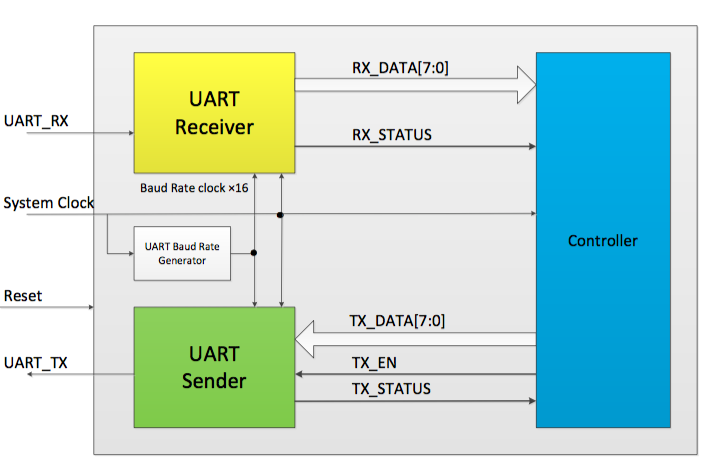
\includegraphics[width=\textwidth]{structure}
  \caption{串口收发器功能实现框图}
  \label{fig:串口收发器功能实现框图}
\end{figure}


\section{关键代码}

\subsection{采样器状态机部分的实现}

\begin{minted}[bgcolor=bg, linenos=true, fontsize=\footnotesize]{verilog}
reg [1:0] state, next_state;
localparam STANDING_BY = 2'd0,
           PADDING = 2'd1,
           SAMPLING = 2'd2;

// Assume SAMPLE_RATIO <= 16
reg [3:0] count = 0, next_count,
          bit_count = 0, next_bit_count;
wire next_sample_sig;

// Calculate next values.
always @(*) begin
    case (state)
    STANDING_BY: begin
        next_state = (din ? STANDING_BY : PADDING);
        next_count = 4'b0;
        next_bit_count = 4'b0;
    end

    PADDING: begin  // Wait PADDING_TIME clk.
        if (count < PADDING_TIME - 1) begin
            next_state = PADDING;
            next_count = count + 4'b1;
        end else begin
            next_state = SAMPLING;
            next_count = 4'b0;
        end
        next_bit_count = 4'b0;
    end

    SAMPLING: begin  // Cycle = SAMPLE_RATIO.
        next_state = (bit_count == 4'd9 ? STANDING_BY : SAMPLING);

        if (count < SAMPLE_RATIO - 1) begin
            next_count = count + 4'b1;
            next_bit_count = bit_count;
        end else begin
            next_count = 4'b0;
            next_bit_count = bit_count + 4'b1;
        end
    end

    default: begin
        next_state = 0;
        next_count = 0;
        next_bit_count = 0;
    end
    endcase
end

assign next_sample_sig = (state == SAMPLING &&
                          count == SAMPLE_RATIO - 4'd2 &&
                          bit_count < 4'd8);

// Update values.
always @(posedge sample_clk) begin
    state <= next_state;
    count <= next_count;
    bit_count <= next_bit_count;
    sample_sig <= next_sample_sig;
end
\end{minted}


\subsection{接受器的实现}

\begin{minted}[bgcolor=bg, linenos=true, fontsize=\footnotesize]{verilog}
// 1 padding, 1 start-bit, 8 data-bits, 1 end-bit.
localparam COUNTER_MAX = 4'd11;

reg [8:0] shift_reg;
assign dout = shift_reg[0];

reg [3:0] counter = 0;
wire rst_n = ~tx_en;

always @(posedge send_clk or negedge rst_n) begin
    if(~rst_n) begin
        counter <= 0;
    end else begin
        if (counter == 4'b0)
            shift_reg <= {tx_data, 1'b0};  // Load data.
        else
            shift_reg <= {1'b1, shift_reg[8:1]};  // Shift.

        if (counter < COUNTER_MAX)
            counter <= counter + 4'b1;
        else
            counter <= counter;
    end
end

always @(posedge clk) begin
    tx_status <= (counter < COUNTER_MAX ? 1'b0 : 1'b1);
end
\end{minted}


\section{文件清单}

\begin{Verbatim}[fontsize=\scriptsize]
exp4
└── serial_transceiver
    ├── Makefile
    ├── hex_led.v
    ├── receiver.v
    ├── receiver_tb.v
    ├── sampler.v
    ├── sampler_tb.v
    ├── sender.v
    ├── sender_tb.v
    ├── serial_transceiver.bit
    ├── serial_transceiver.ucf
    ├── serial_transceiver.v
    ├── serial_transceiver_tb.v
    └── sim

common
├── bcd7.v
└── watchmaker.v
\end{Verbatim}

其中 Makefile 用来构建仿真程序,sim 文件为 Icarus Verilog 生成的仿真程序。


\section{仿真结果及分析}
使用的仿真工具为:Icarus Verilog 0.9.7。

仿真结果如下:

\VerbatimInput[fontsize=\scriptsize, numbers=left]
{../../exp4/serial_transceiver/result.txt}


\section{综合情况}
见附页。

\section{硬件调试情况}


Cheers \textasciitilde

\includepdf[pages={-}]{serial_transceiver.pdf}

\end{document}

